\documentclass[12pt]{article}
\usepackage{geometry}                % See geometry.pdf to learn the layout options. There are lots.
\geometry{letterpaper}                   % ... or a4paper or a5paper or ... 
%\geometry{landscape}                % Activate for for rotated page geometry
%\usepackage[parfill]{parskip}    % Activate to begin paragraphs with an empty line rather than an indent
\usepackage{graphicx}
\usepackage{amssymb}
\usepackage{/Library/Frameworks/R.framework/Resources/share/texmf/Sweave}

\title{Intraspecific variation influences community network structure: Tracing the roots of interactions to genetics.}
\author{M.K. Lau, R. Michalet and J.P. Malouf}
%\date{}                                           % Activate to display a given date or no date

\begin{document}
\maketitle

\setcounter{tocdepth}{3}
\tableofcontents

\begin{enumerate}
\item Main Question: Does selection produce ecological network
  nestedness? Or, is nestedness primarily a statistical artifact
  (i.e. more abundance species will be more connected and typically
  there is an asymptotic shape of ordered species abundance)?
\item How does this analysis parallel more common analyses of
  diversity?
\item Read the Geum papers    
\item Other things to try:
  \begin{enumerate}
  \item Can we look at the inter-connectedness of cushions based on
    significantly similar? or different communities?
  \end{enumerate}
\end{enumerate}

\subsection{Questions}

\begin{itemize}
  \item Do the most numerically abundant species have the most
    connections?
  \item What traits would increase or decrease the diversity of
    beneficiary species (i.e. facilitation connections)?
\end{itemize}


%%NOTES FROM MEETING WITH RICHARD AND YOANN:
%%2) Caviarres 2009
%%3) Xia Xiao 2009 or 2010
%%4) What are the ecological consequences? Diversity, evolution,
%%response to climate change?
%%5) NOTE that for Astragalus the edge of the cushion was the
%%available habitat.
%%6) Check how negative RII are being handled
%%7) Incorporate the O. corunta phenotype groups. Get the individual
%%abudnance thresholds from Richard.Flower data indicates reproductive success. For both Geum and
%%Onobrychis there is an asymptotic decrease of flower production with
%%increasing beneficiary abundance. In addition for both species there
%%is an distinct grouping of beneficiary abundance into phenotypic
%%classes with tighter cushions having fewer beneficiaries.
%%8) Look at species covariance networks using the co-occurrence data,
%%especially Bromus which is likely a competitive species that
%%excludes others.
%%9) Consider modeling all the data together in a tri-partite network

%%Papers to read:
%%Caviarres papers
%%Geum paper Ecology Letters
%%Xia Xiao's paper from geum
%%Schob (Spain) cost and benefit of facilitation
%%Brad's SEM paper and the Nature paper

\section{Individual level facitilation network models}



\subsection{Dependent Functions}

\begin{Schunk}
\begin{Soutput}
gdata: read.xls support for 'XLS' (Excel 97-2004) files ENABLED.

gdata: read.xls support for 'XLSX' (Excel 2007+) files ENABLED.
\end{Soutput}
\begin{Soutput}
----------------------------------------------------------
This is bipartite 1.14. 
For latest additions type: ?bipartite.
For citation please type: citation("bipartite").
Have a nice time plotting and analysing two-mode networks.
----------------------------------------------------------
\end{Soutput}
\begin{Soutput}
     Tools for Social Network Analysis
Version      2.2-0 created on      2010-11-21.
copyright (c) 2005, Carter T. Butts, University of California-Irvine
Type help(package="sna") to get started.
\end{Soutput}
\end{Schunk}

\subsection{Generate Network Models}

\subsection*{No Test for Significance}
%%Onobrychis cornuta


\subsection{Figures}


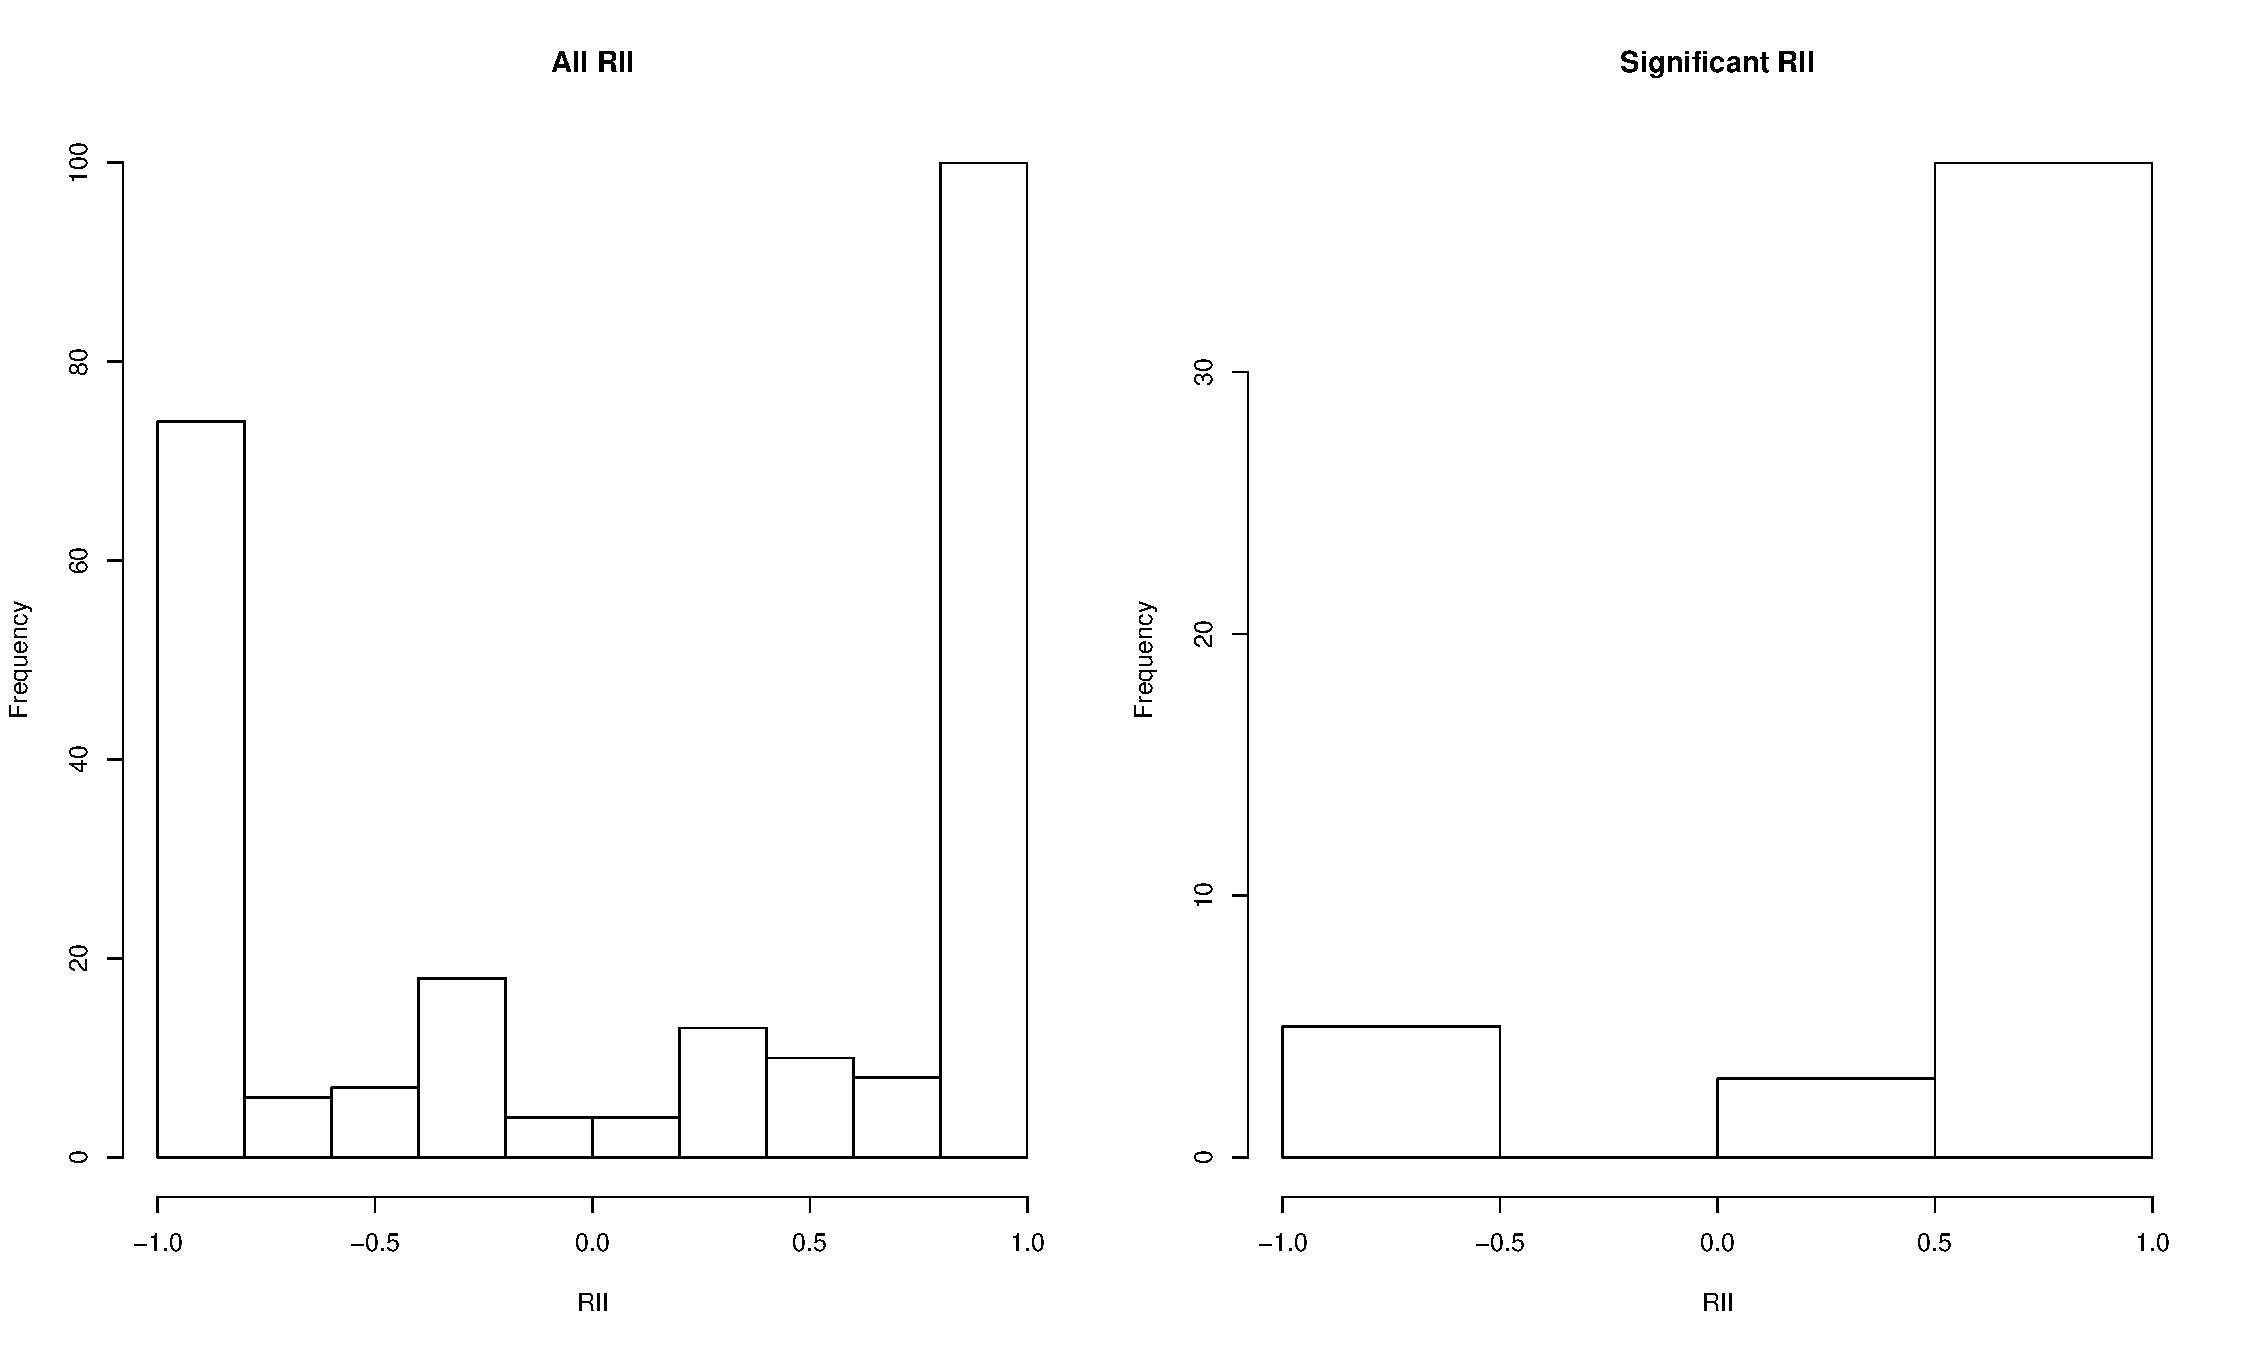
\includegraphics{O_cornuta_ms-004}

\begin{Schunk}
\begin{Soutput}
Checkerboard Units    : 4454 
C-score (species mean): 23.44211 
\end{Soutput}
\begin{Soutput}
Checkerboard Units    : 297 
C-score (species mean): 1.563158 
\end{Soutput}
\begin{Soutput}
oecosimu with 1000 simulations
simulation method quasiswap
alternative hypothesis: true mean is less than the statistic

Checkerboard Units    : 4454 
C-score (species mean): 23.44211 

           statistic          z         0%        50%  95% Pr(sim.)
statistic 4454.00000    0.58601 4172.00000 4397.00000 4556   0.2567
\end{Soutput}
\begin{Soutput}
oecosimu with 1000 simulations
simulation method quasiswap
alternative hypothesis: true mean is less than the statistic

Checkerboard Units    : 4454 
C-score (species mean): 23.44211 

           statistic          z         0%        50%  95% Pr(sim.)
statistic 4454.00000    0.53066 4192.00000 4400.00000 4566   0.2897
\end{Soutput}
\begin{Soutput}
     [,1] [,2]   
[1,] "D"  "RED"  
[2,] "I"  "BLACK"
[3,] "L"  "GREEN"
\end{Soutput}
\end{Schunk}


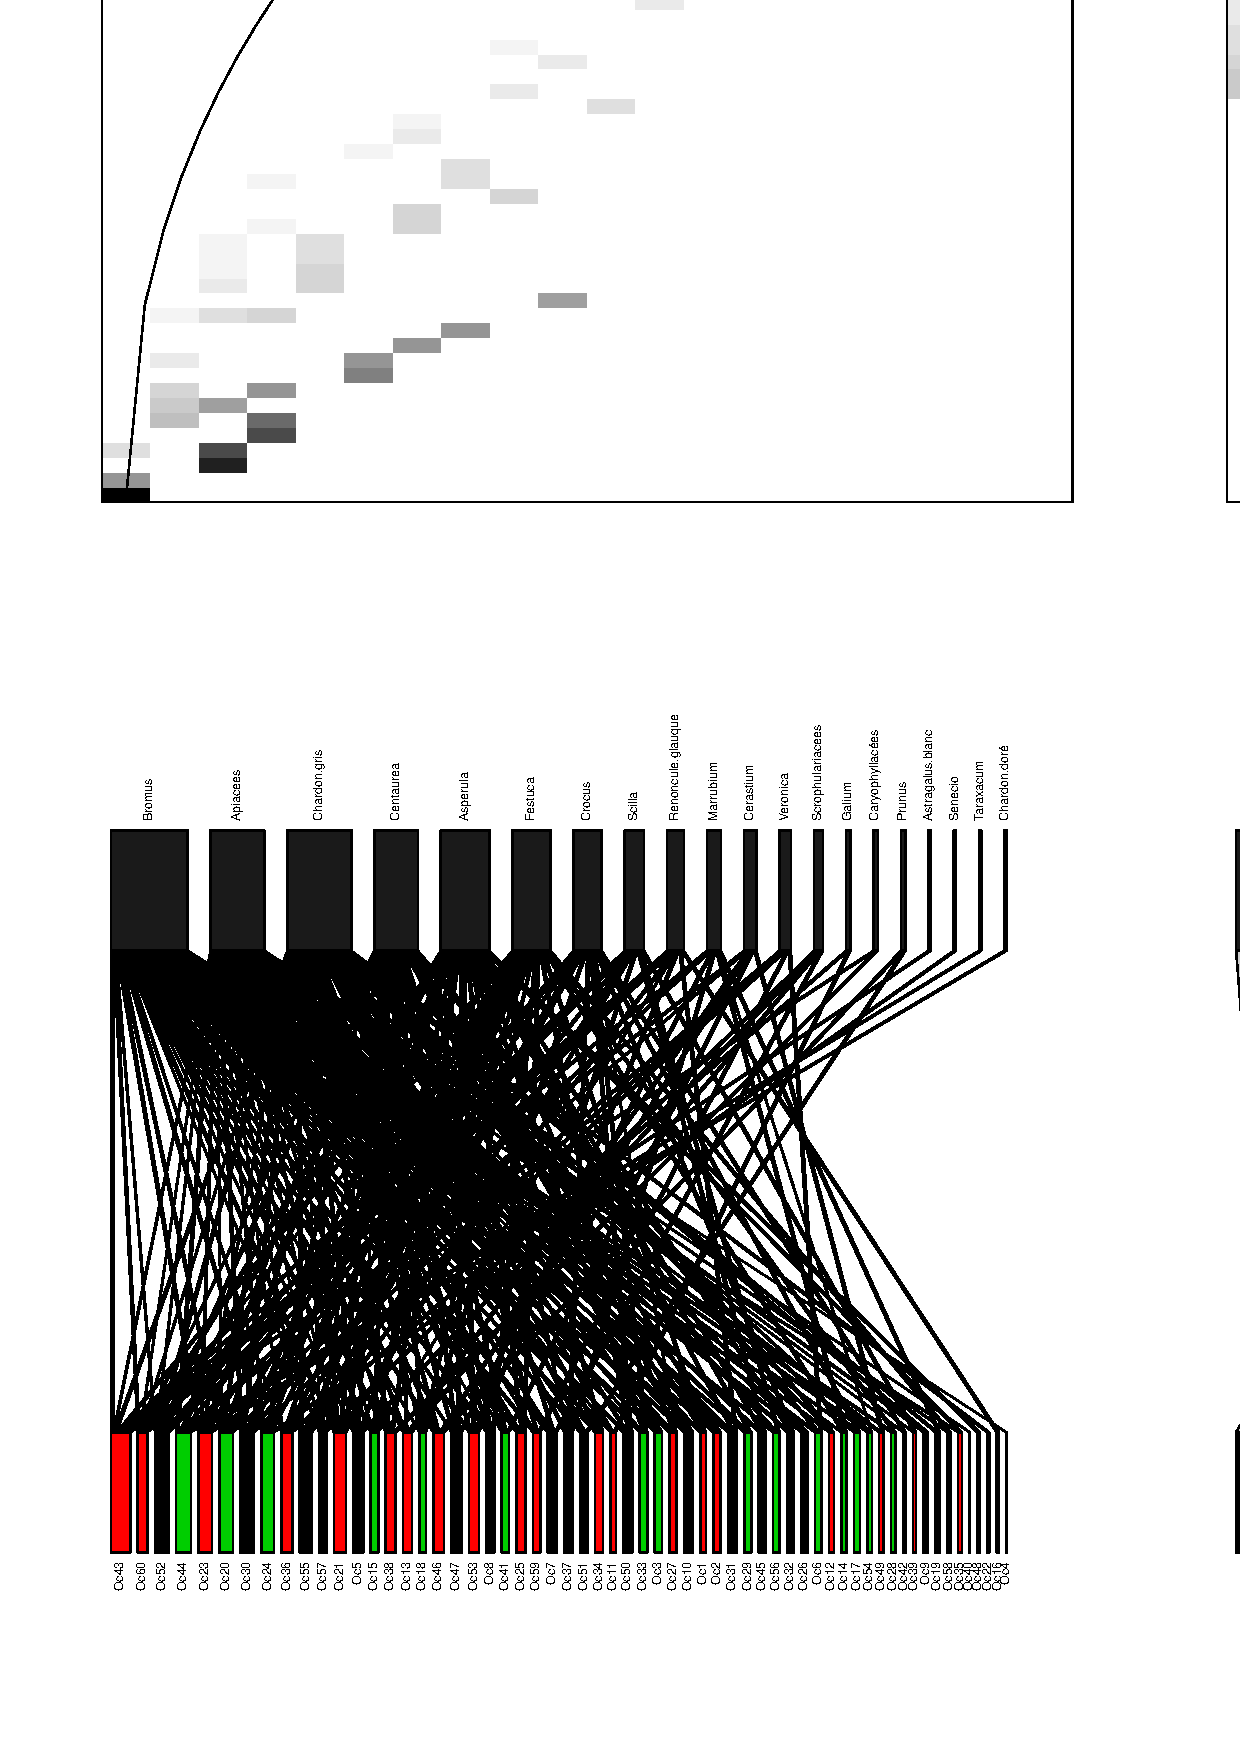
\includegraphics{O_cornuta_ms-006}



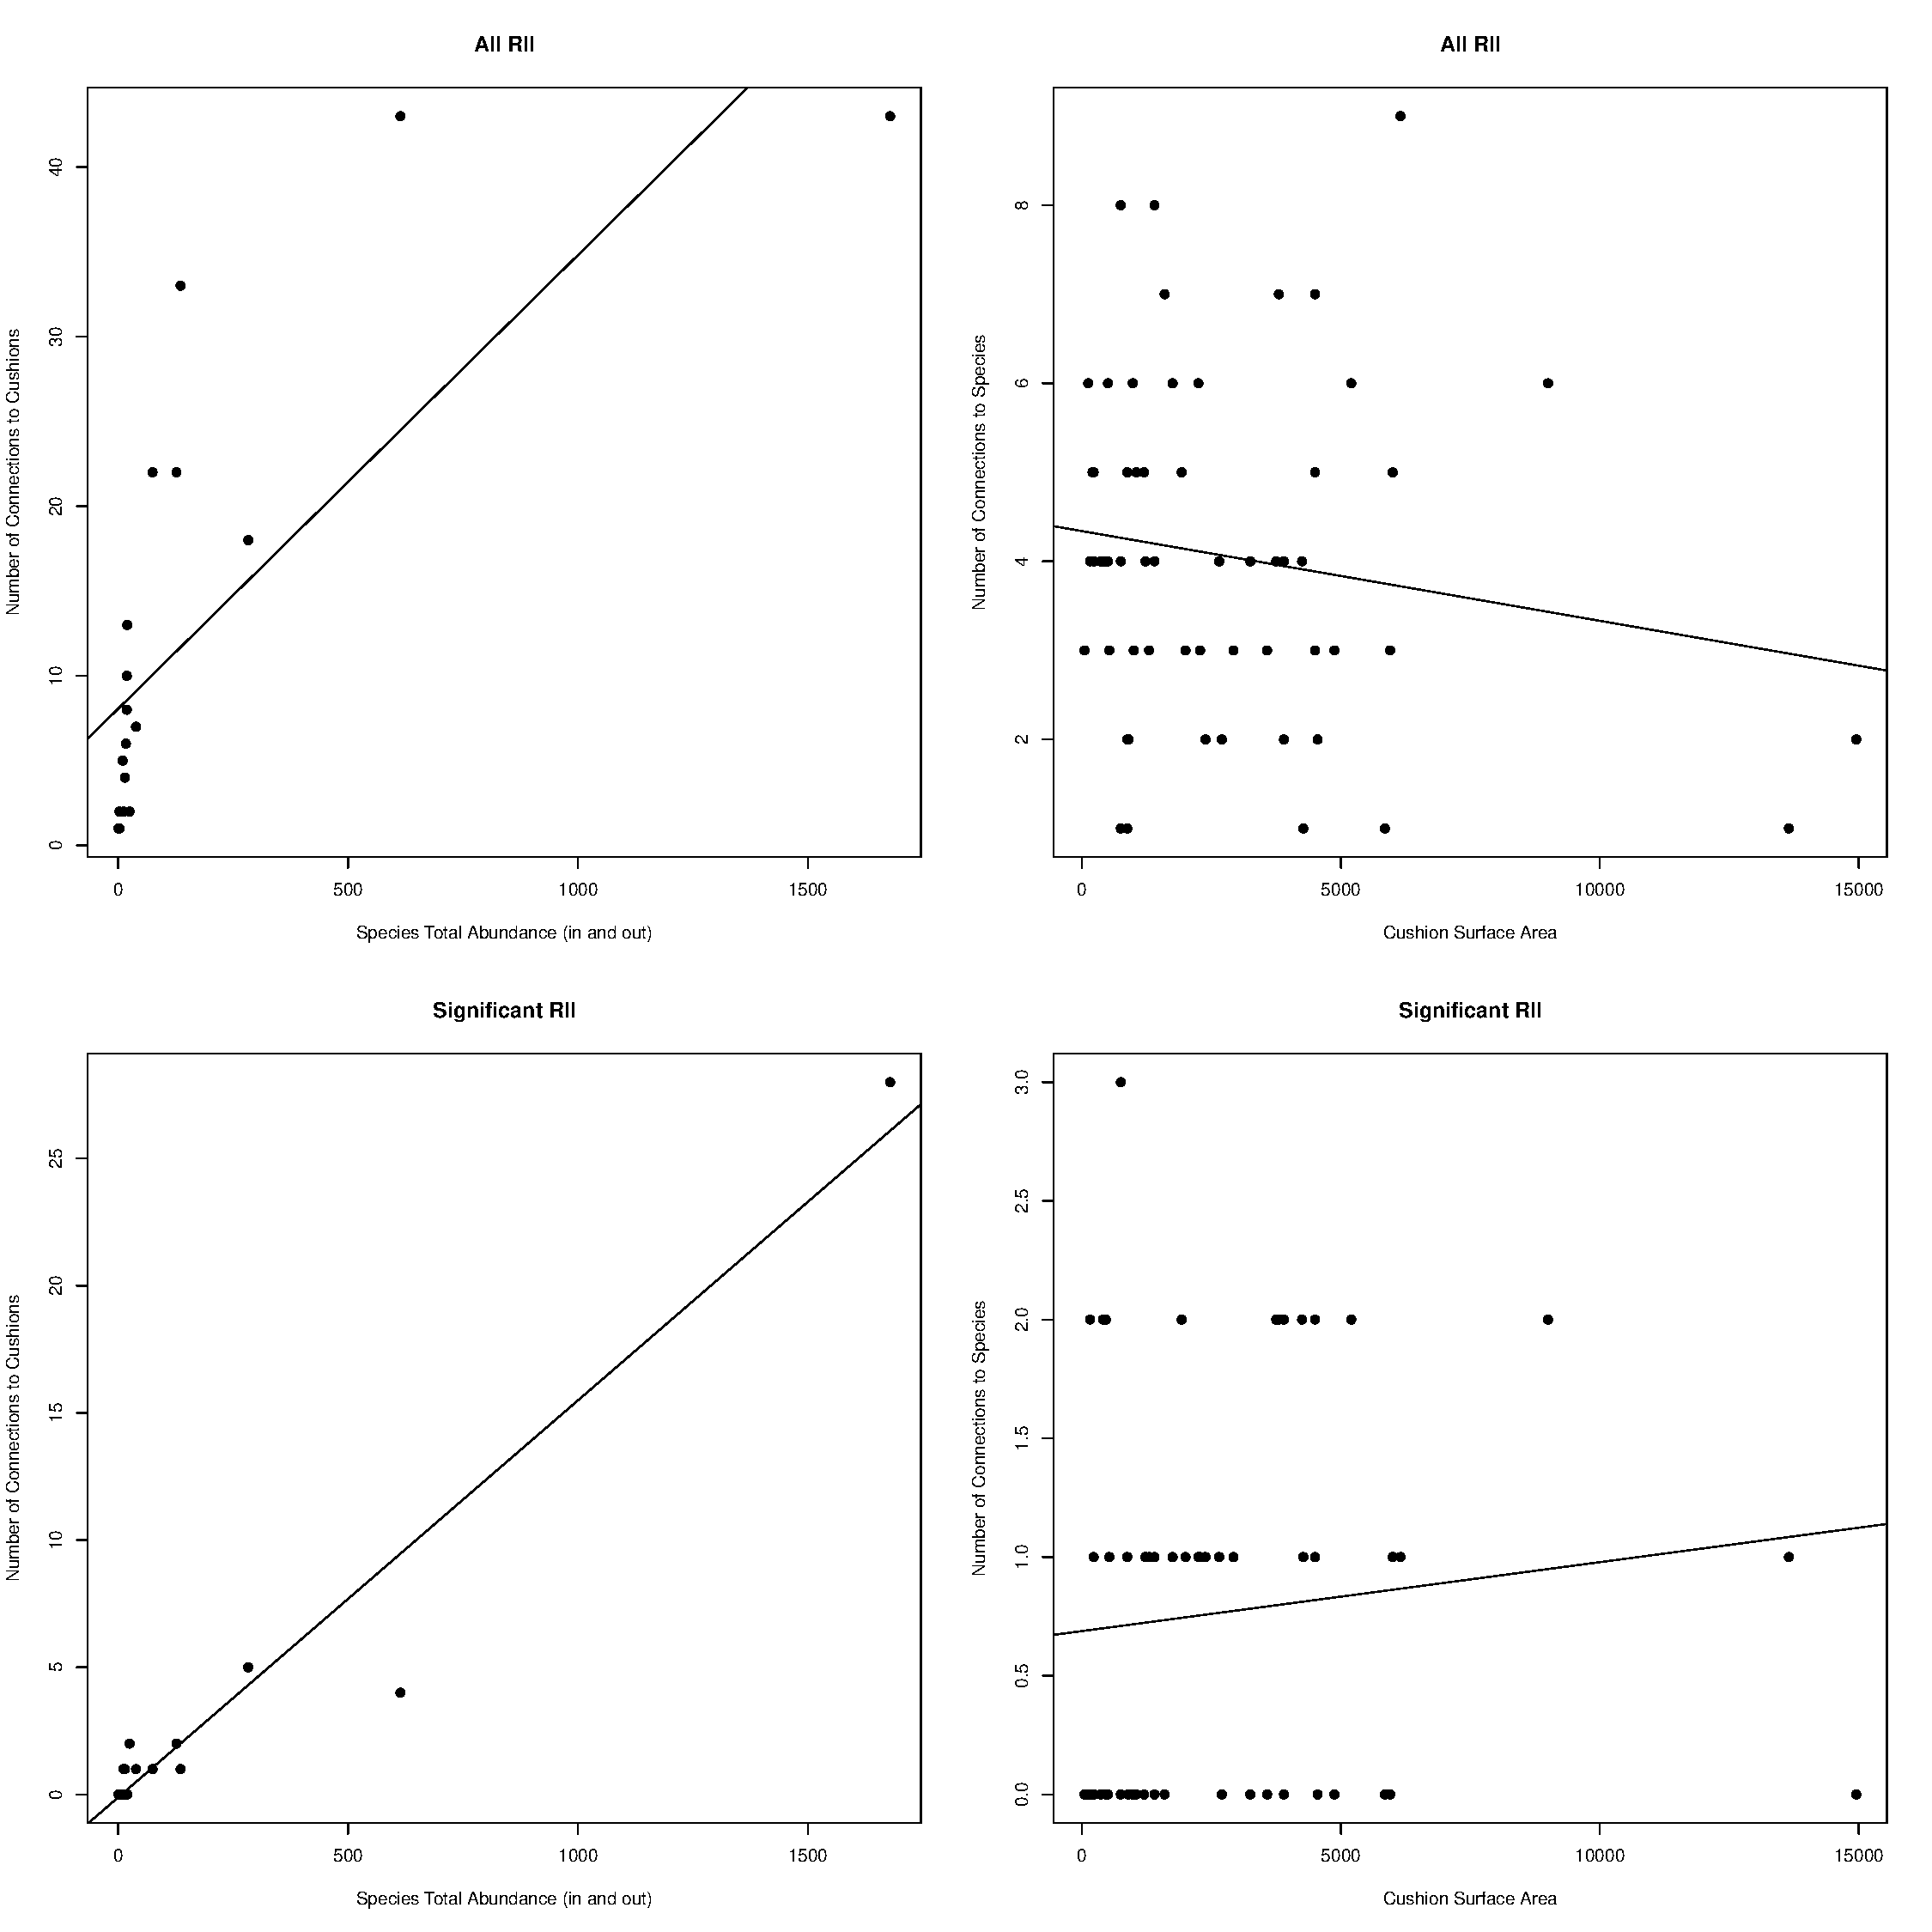
\includegraphics{O_cornuta_ms-008}


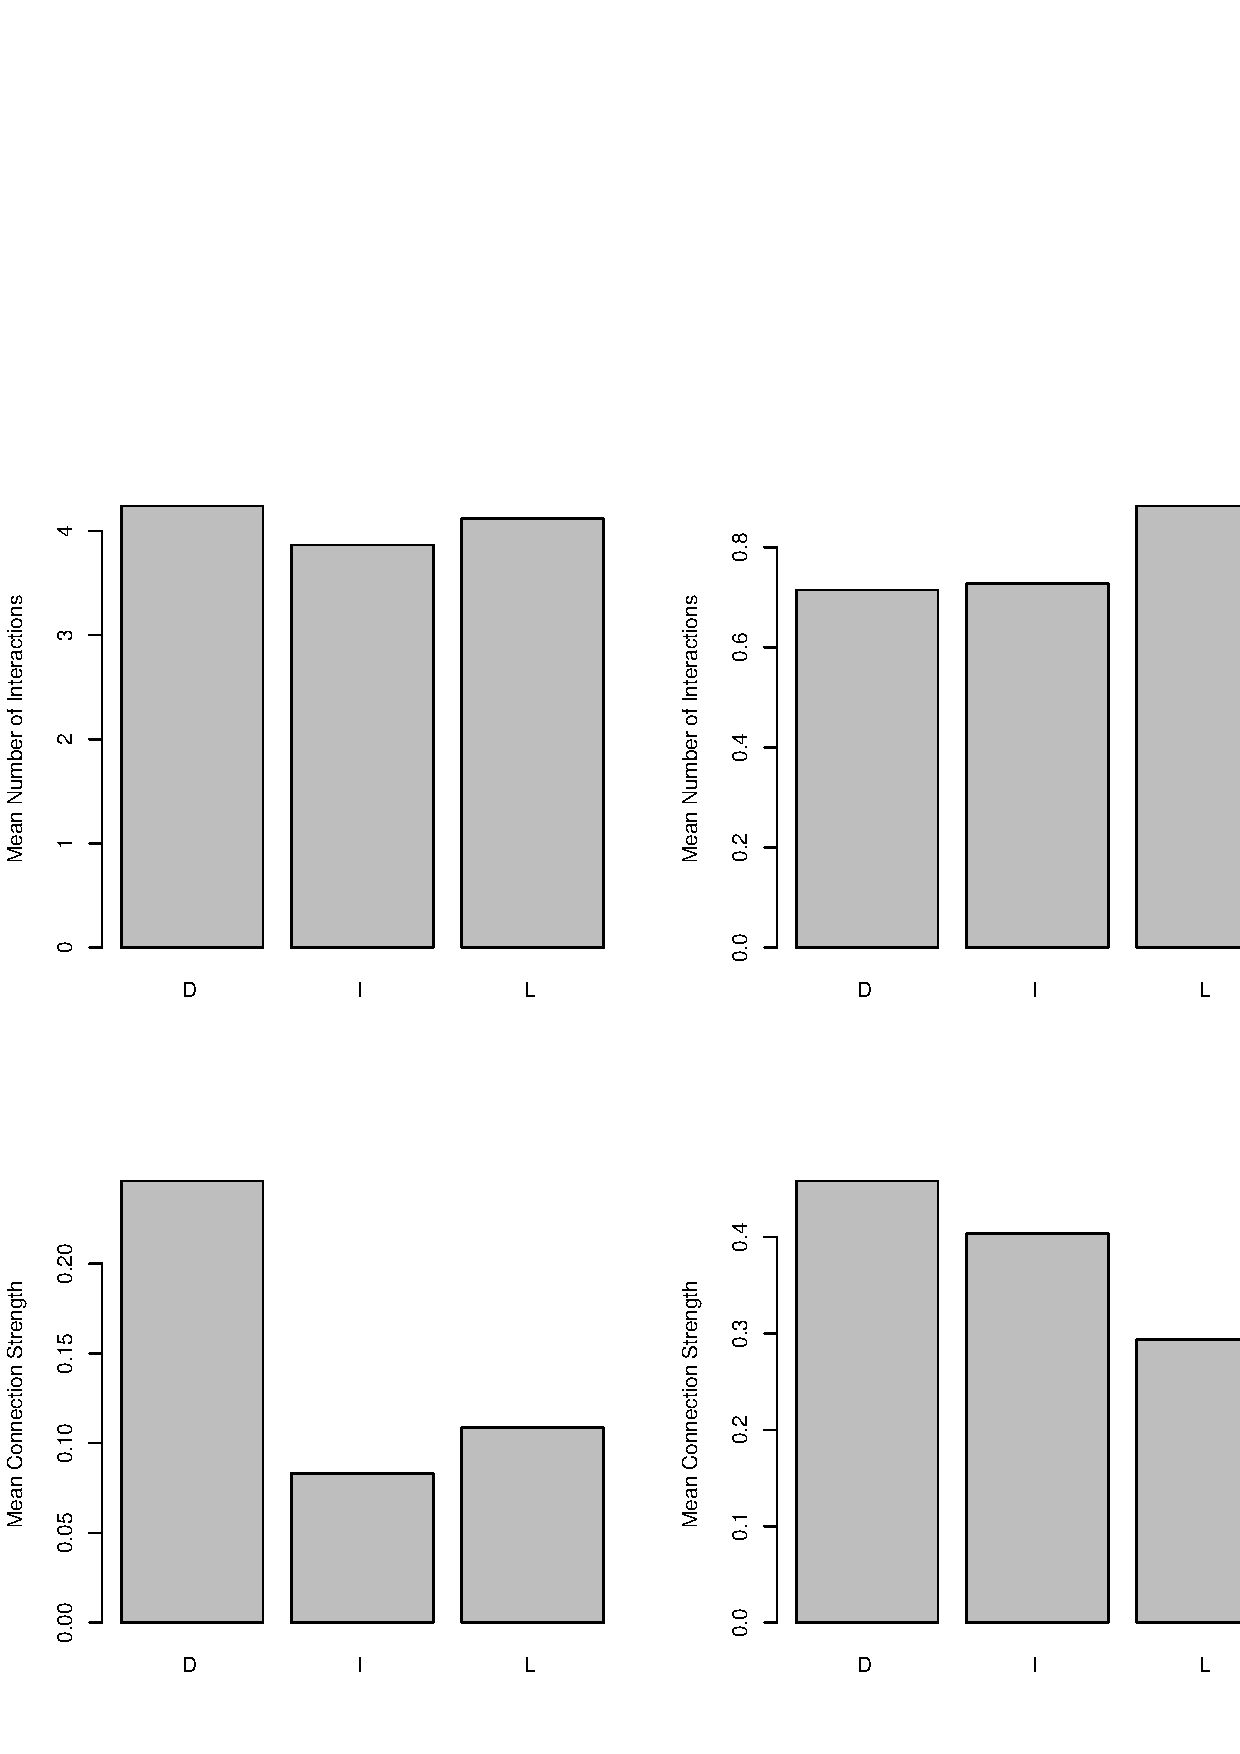
\includegraphics{O_cornuta_ms-010}

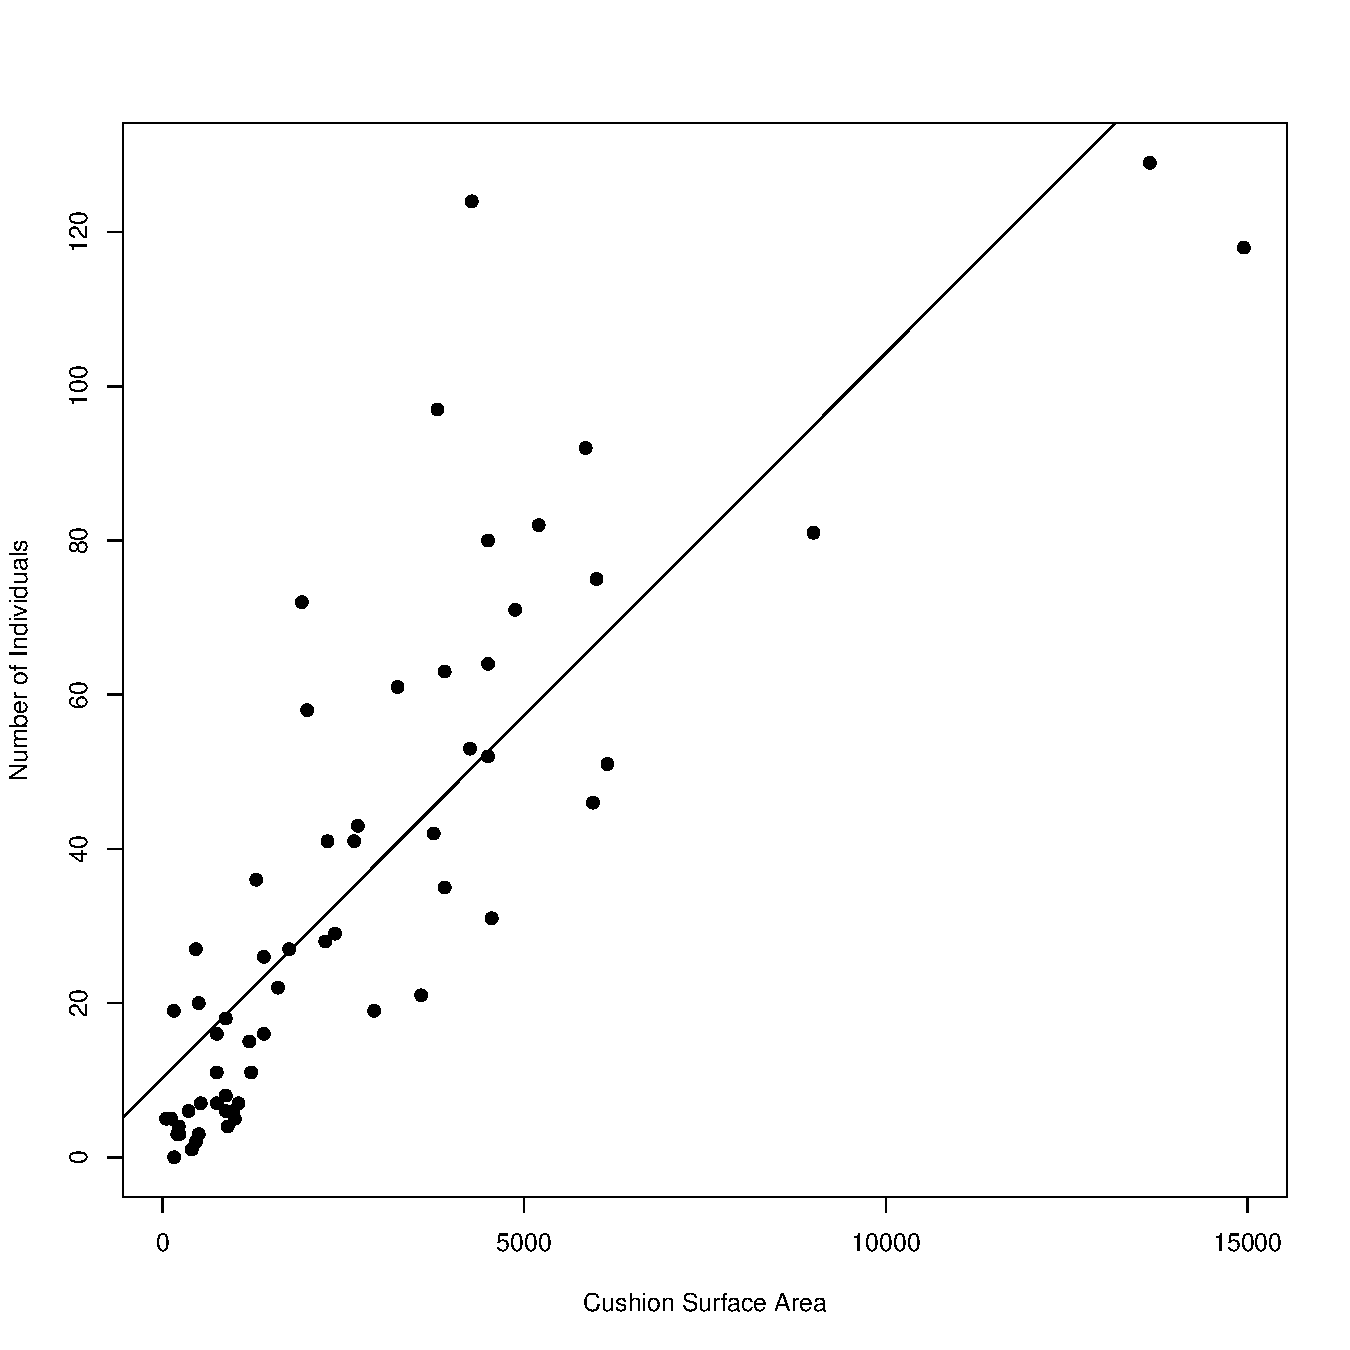
\includegraphics{O_cornuta_ms-011}

\begin{Schunk}
\begin{Soutput}
[1] TRUE
\end{Soutput}
\end{Schunk}
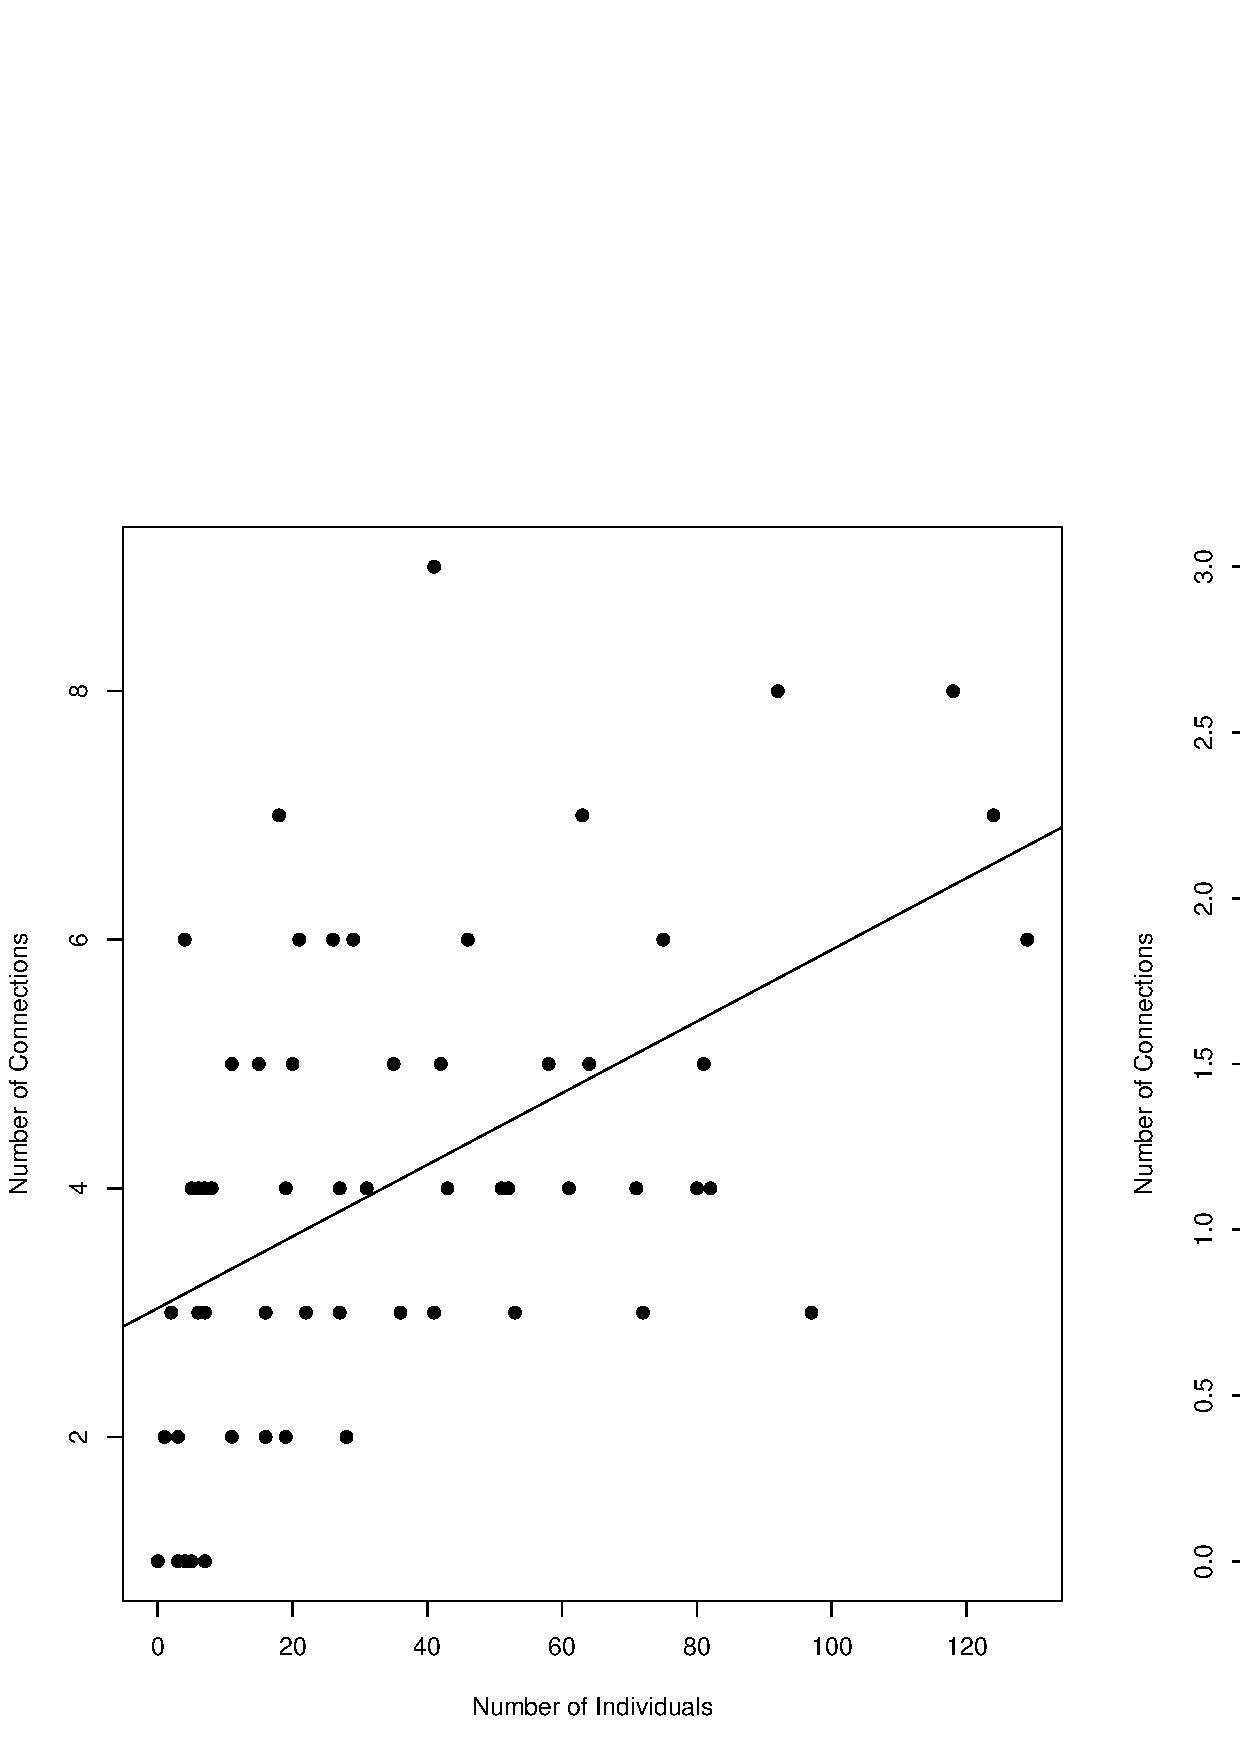
\includegraphics{O_cornuta_ms-012}


% latex table generated in R 2.12.1 by xtable 1.5-6 package
% Tue Oct 18 15:58:33 2011
\begin{table}[ht]
\begin{center}
\begin{tabular}{rrrrr}
  \hline
 & Estimate & Std. Error & t value & Pr($>$$|$t$|$) \\ 
  \hline
(Intercept) & 3.0359 & 0.3040 & 9.99 & 0.0000 \\ 
  Oc.ind & 0.0288 & 0.0062 & 4.63 & 0.0000 \\ 
   \hline
\end{tabular}
\end{center}
\end{table}% latex table generated in R 2.12.1 by xtable 1.5-6 package
% Tue Oct 18 15:58:33 2011
\begin{table}[ht]
\begin{center}
\begin{tabular}{rrrrr}
  \hline
 & Estimate & Std. Error & t value & Pr($>$$|$t$|$) \\ 
  \hline
(Intercept) & 0.1344 & 0.1059 & 1.27 & 0.2095 \\ 
  Oc.ind & 0.0177 & 0.0022 & 8.15 & 0.0000 \\ 
   \hline
\end{tabular}
\end{center}
\end{table}
\section{Facilitation vs Exclusion}

Bromus seems to be the most highly facilitated species, although this
could be because it's the most numerically abundant.

\begin{Schunk}
\begin{Sinput}
> Oc.fac <- apply(Oc.order, 2, function(x) length(x[x > 0]))
> Oc.exc <- apply(Oc.order, 2, function(x) length(x[x < 0]))
> barplot(rbind(Oc.fac, Oc.exc), beside = TRUE, las = 2)
> Oc.fac
\end{Sinput}
\begin{Soutput}
           Bromus          Apiacees      Chardon.gris         Centaurea 
               37                13                13                10 
         Asperula           Festuca            Crocus            Scilla 
                4                15                 6                 4 
Renoncule.glauque         Marrubium         Cerastium          Veronica 
                7                 7                 5                 5 
 Scrophulariacees            Galium   Caryophyllacées            Prunus 
                4                 2                 1                 1 
 Astragalus.blanc           Senecio         Taraxacum      Chardon.doré 
                0                 0                 1                 0 
\end{Soutput}
\begin{Sinput}
> Oc.fac.. <- apply(Oc.order.., 2, function(x) length(x[x > 0]))
> Oc.exc.. <- apply(Oc.order.., 2, function(x) length(x[x < 0]))
> barplot(rbind(Oc.fac.., Oc.exc..), beside = TRUE, las = 2)
> Oc.fac..
\end{Sinput}
\begin{Soutput}
           Bromus           Festuca          Apiacees         Centaurea 
               27                 5                 2                 2 
           Galium      Chardon.gris  Scrophulariacees         Marrubium 
                2                 0                 1                 1 
         Asperula            Prunus         Cerastium          Veronica 
                0                 1                 0                 0 
Renoncule.glauque            Crocus            Scilla  Astragalus.blanc 
                0                 0                 0                 0 
          Senecio   Caryophyllacées         Taraxacum      Chardon.doré 
                0                 0                 0                 0 
\end{Soutput}
\begin{Sinput}
> par(mfrow = c(1, 2))
> barplot(rbind(Oc.fac, Oc.exc), beside = TRUE, las = 2)
> barplot(rbind(Oc.fac.., Oc.exc..), beside = TRUE, las = 2)
\end{Sinput}
\end{Schunk}

\begin{Schunk}
\begin{Sinput}
> Oc.l <- list()
> Oc.l[[1]] <- Oc.com[Oc.env$microsite == "in open", ]
> Oc.l[[2]] <- Oc.com[Oc.env$microsite == "on cushion", ]
> names(Oc.l) <- levels(Oc.env$microsite)
> Oc.net <- list()
> Oc.net[[1]] <- kendall.pairs(Oc.l[[1]], adj.method = "fdr", p.adj = FALSE)
> Oc.net[[2]] <- kendall.pairs(Oc.l[[2]], adj.method = "fdr", p.adj = FALSE)
> names(Oc.net) <- names(Oc.l)
> gplot(abs(Oc.net[[1]]), displaylabels = TRUE, main = "In Open", 
+     label.cex = 0.5)
> gplot(abs(Oc.net[[2]]), displaylabels = TRUE, main = "On Cushion", 
+     label.cex = 0.5)
\end{Sinput}
\end{Schunk}

\section{Conduct module detection and then see if there is overlap
  with the cushion phenotype}

\begin{Schunk}
\begin{Sinput}
> Oc.bg <- graph.incidence(incidence = as.matrix(Oc.order))
> Oc.bg. <- graph.incidence(incidence = as.matrix(Oc.order..))
> clusters(Oc.bg)
\end{Sinput}
\begin{Soutput}
$membership
 [1] 0 0 0 0 0 0 0 0 0 0 0 0 0 0 0 0 0 0 0 0 0 0 0 0 0 0 0 0 0 0 0 0 0 0 0 0 0 0
[39] 0 0 0 0 0 0 0 0 0 0 0 0 0 0 0 0 0 0 0 0 0 0 0 0 0 0 0 0 0 0 0 0 0 0 0 0 0 0
[77] 0 0 0 0

$csize
[1] 80

$no
[1] 1
\end{Soutput}
\begin{Sinput}
> clusters(Oc.bg.)
\end{Sinput}
\begin{Soutput}
$membership
 [1]  0  0  0  0  0  0  0  0  0  0  0  0  0  0  0  1  0  0  0  0  0  0  0  0  0
[26]  0  0  0  0  0  0  0  0  2  3  4  5  6  7  8  9 10 11 12 13 14 15 16 17 18
[51] 19 20 21 22 23 24 25 26 27 28  0  0  0  0  0  0  0  1  0  0 29 30 31 32 33
[76] 34 35 36 37 38

$csize
 [1] 41  2  1  1  1  1  1  1  1  1  1  1  1  1  1  1  1  1  1  1  1  1  1  1  1
[26]  1  1  1  1  1  1  1  1  1  1  1  1  1  1

$no
[1] 39
\end{Soutput}
\end{Schunk}

\section{Examine the monopartite structure and groupings by phenotype}

\begin{Schunk}
\begin{Sinput}
> Oc.om <- as.one.mode(Oc.order, project = "lower")
> Oc.om. <- as.one.mode(Oc.order.., project = "lower")
> par(mfrow = c(2, 2))
> gplot(abs(Oc.om), displaylabels = TRUE, gmode = "graph", vertex.col = as.numeric(factor(Oc.pheno)))
> gplot(abs(Oc.om.), displaylabels = TRUE, gmode = "graph", vertex.col = as.numeric(factor(Oc.pheno..)))
> legend("topright", legend = sort(unique(Oc.pheno)), pch = 19, 
+     col = as.numeric(factor(sort(unique(Oc.pheno)))), box.lwd = 0.5)
> Bs.om <- as.one.mode(Oc.order, project = "higher")
> Bs.om. <- as.one.mode(Oc.order.., project = "higher")
> gplot(abs(Bs.om), displaylabels = TRUE, gmode = "graph")
> gplot(abs(Bs.om.), displaylabels = TRUE, gmode = "graph")
> Bs.n <- Bs.om
> Bs.n[Bs.n > 0] <- 0
> Bs.n. <- Bs.om.
> Bs.n.[Bs.n. > 0] <- 0
> par(mfrow = c(2, 2))
> gplot(abs(Bs.om), displaylabels = TRUE, gmode = "graph")
> gplot(abs(Bs.om.), displaylabels = TRUE, gmode = "graph")
> gplot(abs(Bs.n), displaylabels = TRUE, gmode = "graph")
> gplot(abs(Bs.n.), displaylabels = TRUE, gmode = "graph")
\end{Sinput}
\end{Schunk}
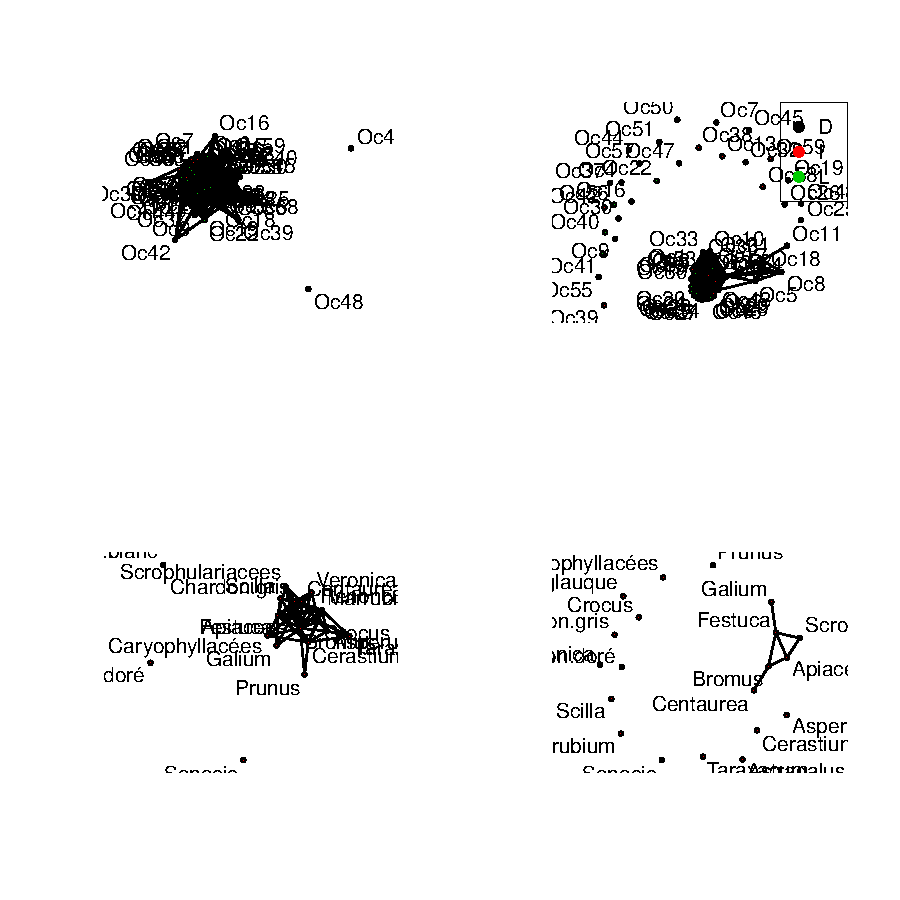
\includegraphics{O_cornuta_ms-017}

\end{document}  



